\section{Теоретическая информация}
\subsection{Метод конфигурационного взаимодействия}
Метод конфигурационного взаимодействия (КВ или CI - configuration interaction) позволяет учесть корреляционные эффекты в молекулярной системе. В данном методе волновая функция раскладывается в ряд по детерминантам Слейтера $\Psi_k$, каждый их которых описывает систему в некотором электронном состоянии. Одно из таких состояний $\Psi_0$ является основным. Остальные состояния описываются электронными конфигурациями, в которых последовательно учтены возможные переходы электронов с занятых МО на различные незанятые (виртуальные) орбитали. Такие состояния также называют возбужденными. Эти состояния классифицируют по числу МО, замещенных виртуальными (одно-, дву, трех-, \ldots, N-кратно замещенные детерминанты). 

Полная волновая КВ-функция, учитывающая все возможные электронные конфигурации, имеет вид
\mequation{
    \Psi_{CI} = a_0\Psi_0 + \sum\limits_{k=1}^{\infty}a_k\Psi_k
}
и находится с помощью вариационного принципа. При этом спин-орбитали в каждом слейтеровском детерминанте $\Psi_k$ остается неизменными в течение всего расчета (их предварительно рассчитывают методом ХФ)\footnote{Однако в более продвинутом методе MCSCF (Multi-Configurational Self-Consistent Field) оптимизируются не только коэффициенты, но и сами спин-орбитали.}.

\begin{figure}[H]
\centering
\captionsetup{justification=centering}
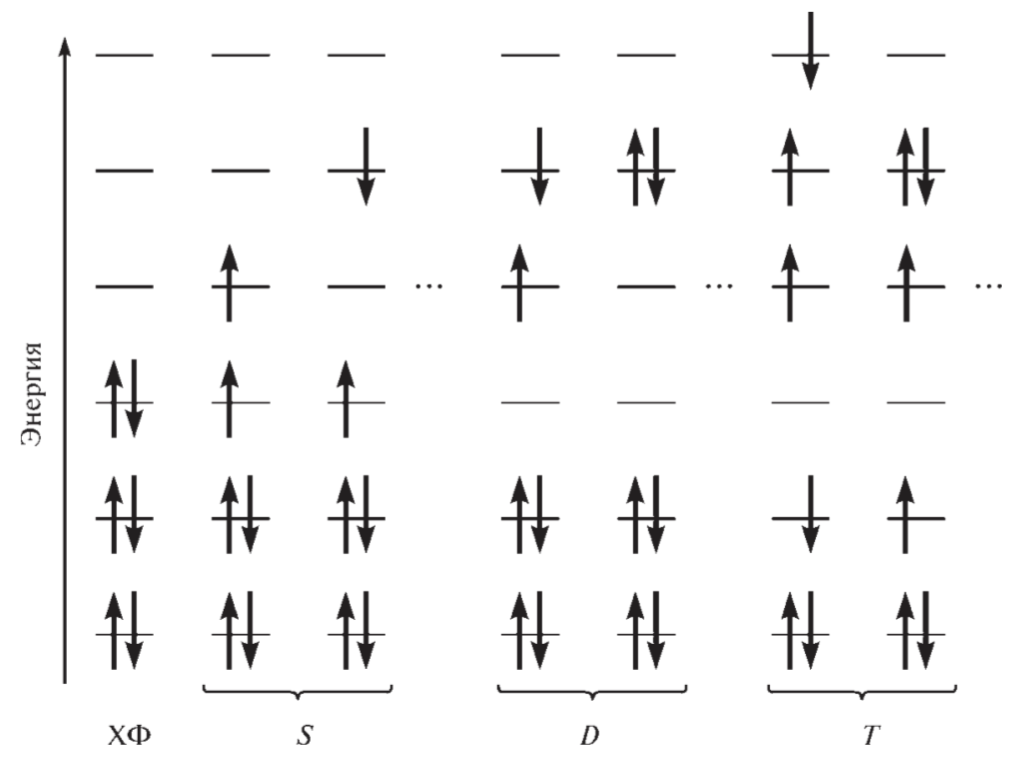
\includegraphics[scale=0.5]{fig/2.png}
\caption{Схема, иллюстрирующая формирование замещенных электронных конфигураций путем перемещения в детерминантах Слейтера электронов с МО, занятых в основном состоянии, на виртуальные МО. ХФ обозначает электронную конфигурацию основного состояния ( полученного методом Хартри—Фока). Буквами S, D и T обозначены одно-, дву- и трехкратно замещенные конфигурации соответственно}
\end{figure}
